%# -*- coding: utf-8-unix -*-
%%==================================================
%% chapter02.tex for SJTU Master Thesis
%% Encoding: UTF-8
%%==================================================

\chapter{电路拓扑符号化自动降阶模型生成方法}
\label{chap:simp}

上一章介绍了电路模型对电路设计的重要性,可见电路低阶模型本身的提出也应有一定方法可以指导其生成。
只有在拥有可靠的模拟集成电路低阶模型的情况下,电路设计工程师才有可能对电路做出进一步的理论分析,从而指导进一步的设计。
本章给出了本文最关键的算法:采用拓扑简化方法得到的低阶模型自动生成算法,并给出了其相关的测试结果,佐证了算法的有效性。

\section{双图决策树符号约简}
\label{sec:simp:GPDD}

\subsection{电路元件极值与元件拓扑的关系}
\label{subsec:simp:GPDD:TopoLimit}

本课题采用拓扑简化的方法实现电路模型的自动生成。
所以电路元件的拓扑结构对于分析本身有非常重要的作用。
我们发现电路的元件的极限取值可以代表新的简化的电路拓扑结构。
这正可以成为我们对电路简化的基石。
当我们考虑需要将一个电路中的元件删去时,即可认为是电路这个元件选取了极限的取值导致。
当然一个电路元件删去过程中,往往存在两个电路元件删去方式:短路和断路。

\begin{figure}[!htp]
	\centering
	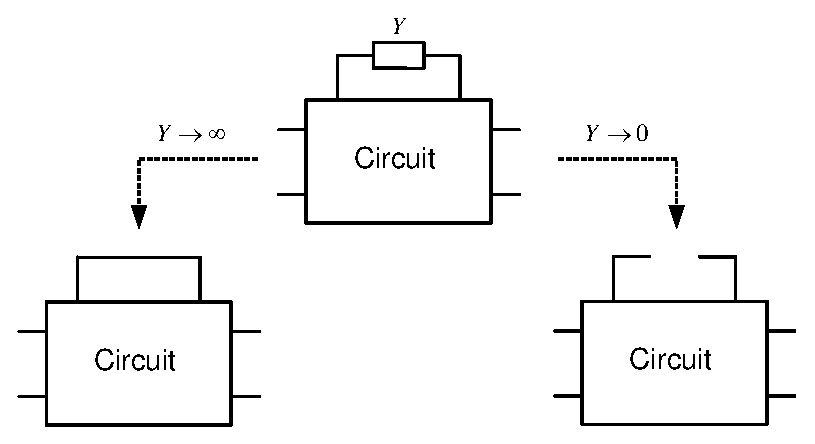
\includegraphics[width=0.7\textwidth]{chap2/LimitTopo.eps}
	\bicaption[fig:limittopo]{导纳在极限取值情况下的拓扑结构改变}{导纳在极限取值情况下的拓扑结构改变}{Fig}{Topological adjustment of impedance whose value changes to limit value}
\end{figure}

如图\ref{fig:limittopo}所示,假设在一个电路中有一处导纳值为$Y$的阻抗。
现在我们用两个极限的值$\infty$和$0$去替代这个导纳值$Y$。
可以看到当,导纳值$Y$趋向于无穷大时,由于此时其相应的阻抗$Z$为零,所以此时这个阻抗变为短路的电路结构;
然而当导纳值$Y$趋向于零时,由于此时其阻抗值$Z$为无穷大,这种情况下电路结构变为阻抗两端的两个节点变为了断路的状态。
可以看到,这样我们就可以用电路元件的极限取值来替代线性阻抗元件(R/L/C)的拓扑变化。

然而,在小信号电路中,我们知道不仅存在线性阻抗元件(R/L/C),另外还有四种受控信号源,分别为:电压控制电压源(VCVS),电流控制电流源(CCCS),电压控制电流源(VCCS),电流控制电压源(CCVS)。
我们发现在以上两种极限取值仍然适用于这四种受控源,特别是在取无穷大情况下,它们都会成为一种称为Nullor的电路元件,如图\ref{fig:nullor}。

\begin{figure}[!htp]
	\centering
	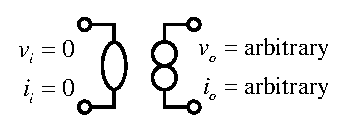
\includegraphics[width=0.35\textwidth]{chap2/SymbolNullor.eps}
	\bicaption[fig:nullor]{Nullor元件符号}{Nullor元件符号}{Fig}{Nullor symbol}
\end{figure}

可以看到,Nullor元件假设其输入端的输入电流和电压均为0,有着任意大小的输出能力。
Nullor这种元件与传统的模拟电路学习中接入负反馈中的理想运算放大器的虚短虚断的性质是一致。
但由于Nullor本身往往可以与电路中别的元件合并,并且不会出现在电路最后的模型中,这一点会在本章中节\ref{subsubsec:simp:res:cir:fd}中看到。

\begin{table}[!htbp]
	\bicaption[tab:symbollimit]{电路元件极限取值的拓扑结构}{电路元件极限取值的拓扑结构}{Table}{Circuit element topology whose value is infinity or zero}
	\centering
	\begin{tabular}{c|c|c}
		\hline
		\multirow{2}{*}{Symbol} & \multicolumn{2}{c}{Value}\\
		\cline{2-3} 
		& $\infty$ & $0$\\
		\hline
		\parbox[c]{0.11\textwidth}{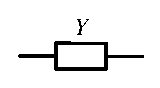
\includegraphics[width=0.11\textwidth]{chap2/Impedance.eps}} & 
		\parbox[c]{0.11\textwidth}{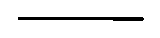
\includegraphics[width=0.11\textwidth]{chap2/Impedance-Short.eps}} & 
		\parbox[c]{0.11\textwidth}{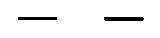
\includegraphics[width=0.11\textwidth]{chap2/Impedance-Open.eps}} \\
		\hline
		\parbox[c]{0.2\textwidth}{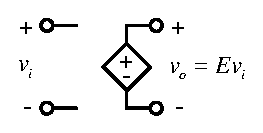
\includegraphics[width=0.2\textwidth]{chap2/VCVS.eps}} & 
		\parbox[c]{0.11\textwidth}{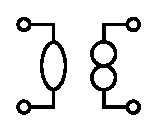
\includegraphics[width=0.11\textwidth]{chap2/Nullor.eps}} & 
		\parbox[c]{0.11\textwidth}{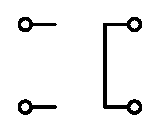
\includegraphics[width=0.11\textwidth]{chap2/VCVS-Open.eps}} \\
		\hline
		\parbox[c]{0.2\textwidth}{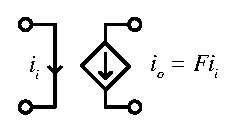
\includegraphics[width=0.2\textwidth]{chap2/CCCS.eps}} & 
		\parbox[c]{0.11\textwidth}{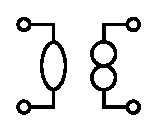
\includegraphics[width=0.11\textwidth]{chap2/Nullor.eps}} & 
		\parbox[c]{0.11\textwidth}{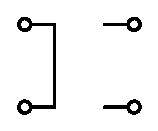
\includegraphics[width=0.11\textwidth]{chap2/CCCS-Open.eps}} \\
		\hline
		\parbox[c]{0.2\textwidth}{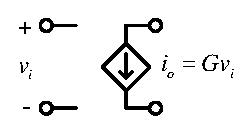
\includegraphics[width=0.2\textwidth]{chap2/VCCS.eps}} & 
		\parbox[c]{0.11\textwidth}{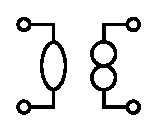
\includegraphics[width=0.11\textwidth]{chap2/Nullor.eps}} & 
		\parbox[c]{0.11\textwidth}{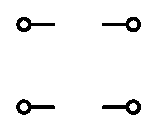
\includegraphics[width=0.11\textwidth]{chap2/VCCS-Open.eps}} \\
		\hline
		\parbox[c]{0.2\textwidth}{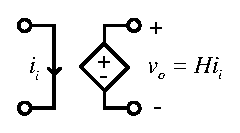
\includegraphics[width=0.2\textwidth]{chap2/CCVS.eps}} & 
		\parbox[c]{0.11\textwidth}{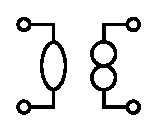
\includegraphics[width=0.11\textwidth]{chap2/Nullor.eps}} & 
		\parbox[c]{0.11\textwidth}{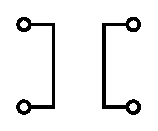
\includegraphics[width=0.11\textwidth]{chap2/CCVS-Open.eps}} \\
		\hline
	\end{tabular}
\end{table}

为了说明受控源取极限值情况下电路拓扑结构的变化,这里仅以VCVS为例进行说明。
所有小信号分析中用到的阻抗和四种受控源的拓扑变化可以参考表\ref{tab:symbollimit}。
我们知道VCVS的输入输出电压关系如下式所示:

\begin{equation}
	v_o = E v_i
\end{equation}

这里,$v_i$和$v_o$分别为VCVS的输入输出电压,$E$则为VCVS的放大倍数。
首先我们考虑$E$取无穷大的情况,为了电路仍然能正常工作,我们知道输出电压$v_o$应为有限值,而其中$E$为无穷大,那么根据基本微积分的知识,我们知道此等式中的输入电压$v_i$为零。
另外由于VCVS的输入端测量电压,所以本来就限定输入的电流$i_i$为零,所以其形成了Nullor的虚短虚断的性质。
另外当$E$的取值为零时,根据VCVS本身的关系,即可得出输出端电压为零,所以输出端两端电压一致,即此端口可用一根导线连接起来,加之本为断路连接的输入端,故VCVS可约减为表\ref{tab:symbollimit}中的结构。

\subsection{双图决策树和电路拓扑的关系}
\label{subsec:simp:GPDD:TopoGPDD}

上一小节已经将电路的极限取值与电路的拓扑结构变化建立起了联系,而此时电路元件的极限求值成为了新的问题。
由于在整个算法过程中,需要多次计算不同拓扑结构下电路性能表现,这要求了高效的计算方法的支持。
然而GPDD结构本身蕴含了对电路拓扑结构,可以轻松方便地在其中对不同的电路拓扑结构求值,这支持了下一节所介绍的简化算法。

\begin{figure}[!htp]
	\centering
	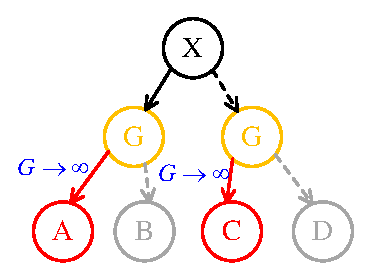
\includegraphics[width=0.35\textwidth]{chap2/GPDDTopo.eps}
	\bicaption[fig:GPDDTopo]{符号极限取值情况下GPDD的计算方法}{符号极限取值情况下GPDD的计算方法}{Fig}{Calculation rule for GPDD under limit value}
\end{figure}

我们知道根据电路基本原理,并且结合GPDD的计算规则,针对类似图\ref{fig:GPDDTopo}这样的GPDD结构,我们可以求得类似下式的电路传输函数表达式(为了说明的方便,这里忽略了GPDD中连接节点的边上的符号):

\begin{equation}
H \left( s \right) = \frac{{{f_A}\left( A \right)G + {f_B}\left( B \right)}}{{{f_C}\left( C \right)G + {f_D}\left( D \right)}}
\end{equation}

考虑目前我们需要对电路中的元件$G$求取极限值,并计算新的符号化传输函数公式。
这里假设元件$G$位于GPDD符号表中的第一层,这里层数不影响极限取值的计算,只是为方便说明特意假设。
我们可以得到在$G$元件取无穷大情况下,电路的新传输函数为:

\begin{equation}
\label{eq:simpGPDD}
\mathop {\lim }\limits_{G \to \infty } H \left( s \right) = \frac{{f_A}\left( A \right)}{{f_C}\left( C \right)}
\end{equation}

首先,十分显然地,可以看到取极限后首先原有的符号$G$从公式消失了,这也暗示了电路拓扑的简化,即$G$从电路中以短路的方式被删去了。
另外,可以发现,在式\ref{eq:simpGPDD}中所有的保留下的符号项均是在GPDD结构中以红色实线相连的红色节点$A$和$C$的值。
由于,我们知道,GPDD结构中实线相连的节点均采用乘法进行计算,故在求取极限的过程中,其相应的系数得到保留。
故当某一符号元件需取无穷大情况下的值时,在GPDD计算过程中,仅需计算GPDD对应符号所有节点左儿子的值即可,所有的右儿子忽略。
同样的,我们知道当对一个电路元件取值零时,GPDD计算中仅需考虑该元件所有节点右儿子的值即可,左儿子的值则忽略,而且算法设计简单,仅需直接用0带入符号值即可。
总结来说,GPDD中某个节点左儿子承担了该节点符号取值无穷大情况(阻抗短路,受控源Nullor)下的电路性能,而右儿子为该节点符号取值零情况(阻抗断路,受控源删去)下的电路性能,当符号本身有一定值时,则为两者的折衷。

当然需要注意的是,在求某一个符号为无穷大时,由于特殊的GPDD规模缩小的算法,类似Reduction、Zero-Suppression等算法\parencite{GShi-GPDD-2013,GShi-GPDD},可能存在有排序在$G$之上的符号直接与排序在$G$之下的符号节点相连的情况。
这种情况需特别注意,因为这种项中不包含$G$符号,故取极限值时,并非系数,也需忽略。
具体的GPDD中符号约减下的计算方法已在\parencite{HanbinHu-Thesis}有阐释,这里不再赘述。

下面通过一个例子展示电路拓扑结构变化对GPDD结构的影响,以直观了解这两者之间的关系。

\begin{exmp}
RLC电路向RC电路简化过程中GPDD结构比较

图\ref{fig:RLC}中展示了一个RLC串联的简易电路,与之前给出的图\ref{fig:RC_cir}相比较,这里多出了电感元件。
可以看到如果这个电感$L$如果取值为零,那么其导纳$Y=\left(s L\right)^{-1}$,即导纳为无穷大情况,即可得到RC电路的电路图。

\begin{figure}[!htp]
	\centering
	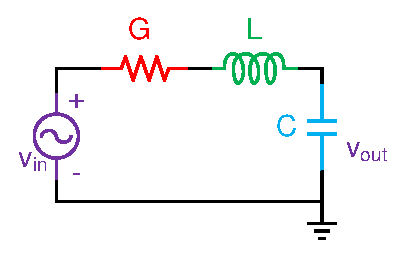
\includegraphics[width=0.4\textwidth]{chap2/RLC.eps}
	\bicaption[fig:RLC]{RLC电路示意图}{RLC电路示意图}{Fig}{RLC circuit example}
\end{figure}

此RLC电路对应的GPDD结构展示在图\ref{fig:RLCvsRC}中的左侧。这张图右侧是展示的RC电路对应的GPDD结构。
可以看到通过两侧曲线包围起来的结构是一致的,而且均与电感符号$L$的左儿子相连,这与之前的论述是相符的。
同时可以看到,由于RC的GPDD结构蕴含在RLC的GPDD结构中,故可以直接在RLC的GPDD结构上对RC电路的GPDD进行求值。
这表示了GPDD拥有在同一个BDD数据结构中求解多种不同电路拓扑的能力,这大大方便了符号简化电路自动生成算法的设计。
这种能在同一个符号化结构中表达不同拓扑结构电路的能力是别的符号化方法不具备的,也是GPDD相比其他的符号化方法一大优势所在。

\begin{figure}[!htp]
	\centering
	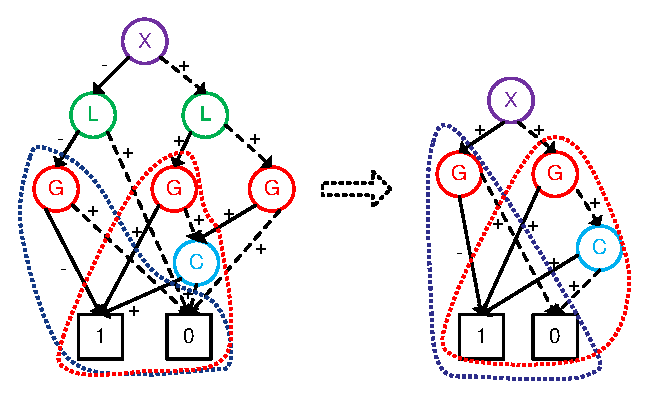
\includegraphics[width=0.7\textwidth]{chap2/RLCvsRC.eps}
	\bicaption[fig:RLCvsRC]{符号极限取值情况下GPDD结构示例}{符号极限取值情况下GPDD结构示例}{Fig}{GPDD structure example under limit value}
\end{figure}

\end{exmp}

GPDD对降阶模型的求解的优势在于在一次符号表达构造的情况下,可以在多次同一个结构中求得对应与不同简化模型的电路传输函数。
符号化构造往往大量计算时间花费在符号化表达式的构造上,而其求值往往是高效的稳定的。
故可以如将构造的时间平摊在之后的多次求值上,仍然得到了许多计算上的便利。
同时,如采用传统的数值化求解器,需要对电路矩阵做行列合并等操作,操作复杂。

\section{符号化降阶模型生成算法与流程}
\label{sec:simp:alg}

在建立电路拓扑与元件取值之间的关系,并使用GPDD这个便利的工具可方便求取电路拓扑变化情况下的电路性能的条件下,本节对符号化降阶模型生成算法进行全面的介绍。
首先,将介绍算法的总体流程,并逐一介绍其中每个流程具体细节,并给出简化过程中一些特殊情况的处理。
本文讨论中,我们主要针对运算放大器的设计进行讨论,故我们接下来的讨论将均针对运算放大器设计。

\subsection{简化算法总体流程}
\label{subsec:simp:alg:top}

降阶模型的建立,我们将其看作一个电路拓扑元件简化的过程,总的流程可参见图\ref{fig:SimpProcedure}的流程示意。

\begin{figure}[!htp]
	\centering
	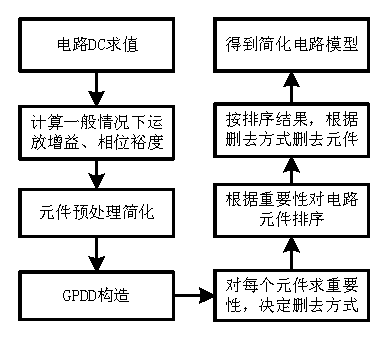
\includegraphics[width=0.5\textwidth]{chap2/SimpProcedure.eps}
	\bicaption[fig:SimpProcedure]{降阶模型自动生成整体流程}{降阶模型自动生成整体流程}{Fig}{Entire procedure for low-order model generation}
\end{figure}

该流程图中有两处以红色斜体标出将在接下来的两个小节\ref{subsec:simp:alg:pre}和\ref{subsec:simp:alg:significance}中详细介绍。
这里先针对其余的部分给出说明。

在拿到一个模拟运放电路后,首先通过数值化仿真器(如:HSPICE)利用DC求解对电路进行求解,以获得电路中所有非线性元件(如:MOSFET)的小信号参数。
接下来,对于完整电路进行AC分析,求得相应的运放增益$A_0$和单位增益频率处相位$PM_0$(即相位裕度处),这两个值将在接下来的元件重要性求值运用到。
对于电路元件进行预处理,做一定粗糙的简化工作,这一步对于生成的最后的简化小信号模型的易于理解性方面有关键的作用,将在\ref{subsec:simp:alg:pre}中具体介绍。
根据初步得到的小信号模型电路,进行GPDD符号化结构的构造,以方便下一步的元件重要性计算。

这里我们定义了电路元件的重要性,某个符号的重要性意味着该电路元件符号对电路性能具有比较大的贡献。
故高重要性的电路元件应予以保留,而低重要性的电路元件应予以删去,故如流程中所示,需要对元件的重要性进行排序。
同时根据前几节的论述,一个符号有两种删去方式,分别为将该元件置为零或无穷大。
我们在计算重要性的过程中即刻确定对应的删去方式,并最终在简化模型生成中以相应的删去方式删去电路元件,从而得到降阶的符号化模型。

这里有一个问题是模型需要多大精度,从而会决定简化的电路模型中保留多少相应的元件。
在目前的研究进程中,我们仅人为指定需要保留多少电路元件,通过人为观察电路频率响应曲线,来决定当前的模型是否合适。

这种简化方法可以看到在符号化构建GPDD后,最关键的时间复杂度主要集中在对元件重要性求值的这一步上。
别的步骤虽然也有一定的时间损耗,但根据我们的实践经验,相比重要性求值步骤来说可以忽略不计。
重要性求值需要对每个电路元件进行计算,故若一个电路中有N个电路元件,构造得到的GPDD结构共有$\left|GPDD\right|$节点。
在\ref{subsec:simp:alg:significance}中可以看到单个元件的重要性求值需$O\left(\left|GPDD\right|\right)$的时间复杂度。
故简化流程的时间复杂度主要由$O\left(N\left|GPDD\right|\right)$决定。

\subsection{元件预处理过程}
\label{subsec:simp:alg:pre}

之所以要对电路进行预先简化,其主要目的在于能够事先将一些信号不通过的节点识别出来,从而事先删去一些节点和元件,方便进一步简化算法。
许多电路从理论上分析,往往会有一定的做法;然而在实际操作中,人们往往会进一步加入自己的理解与分析,从而改变理论分析的结果,虽然过程中隐去了一些电路结构,却使进一步的分析与电路理解更加便利。
这一点在后续的测试结果中也有所体现。
这里以模拟电路中常见的由于输入差分对所造成的虚拟地作为例子,说明这种情况。

\begin{exmp}
虚拟地理论分析与实际操作区别

\begin{figure}[!htp]
	\centering
	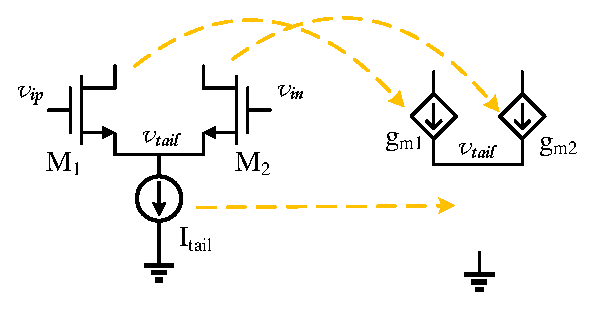
\includegraphics[width=0.6\textwidth]{chap2/VG.eps}
	\bicaption[fig:VG]{虚地的产生原因}{虚地的产生原因}{Fig}{Virtual ground illustration}
\end{figure}

可以看到,图\ref{fig:VG}中展现了经典的模拟电路输入差分对,这样的电路结构一般由一个电流源作为两个输入管的偏置,输入结构两端对称。
在这种结构下,根据传统的电路分析技巧,我们可以画出如图\ref{fig:VG}右侧的小信号结构。
其中理想电流作为断路,所以$v_tail$这一电路节点浮空,同时保留这里的两个MOS管的$g_m$电流源。
我们可以根据$v_tail$这一电路节点的KCL关系,可列写方程有:

\begin{equation}
g_{m1}\left(v_{ip}-v_{tail}\right)+g_{m2}\left(v_{in}-v_{tail}\right)=0
\end{equation}

由于两端的对称性我们知道$v_{ip}=-v_{in}$,并且$g_{m1}=g_{m2}=g_m\neq0$,那么有

\begin{equation}
g_{m} v_{tail} = 0 \Rightarrow v_{tail} = 0
\end{equation}

所以由于尾电流的节点往往被作为虚拟地的存在,在电路分析中往往直接将这一点接到地上,而不是像小信号分析中将电路节点浮空。
这种看似矛盾,实际合理的人为处理结果计算机往往很难自动识别,因为从电路基本理论分析,电路中的电流源应该使用断路的端口进行替代。
即使使用MOS管进行替代,根据传统分析经验,我们知道MOS管往往会近似为一个$r_{ds}$所组成的阻抗,而单一的阻抗并不影响上述分析过程,虚地仍然存在,而往往这个阻抗往往比较大,最后仍然会作为浮空处理。
但这与多数模拟电路工程师的设计经验不符,电路工程师会将类似的结构直接接到地上进行分析。

\end{exmp}

另两种常见的类似电路结构是偏置电路以及镜像电流源。如镜像电流源,往往小信号分析中,作为电流源的MOS管使用电压偏置也并不影响电路的差分工作特性。
造成这种现象的主要原因在于电路信号往往并不直接通过这些节点进行传递,故导致了小信号电路中较低的电压值。
为避免这些电路结构对我们的分析造成影响,我们采取以下的方式对电路进行预处理:

\begin{enumerate}
	\item 求得电路中所有节点的直流处的AC增益。
	\item 将增益最小的节点接地,并删去应删去的元件。(元件的所有端口全接地。)
	\item 如电路的传输相应曲线有较大变化,则终止预处理;否则,回到第2步继续处理。
\end{enumerate}

在这种方案下,我们得到比较合理以及符合工程师习惯的简化电路模型,具体结果可以参照\ref{subsec:simp:res:pre}小节。

\subsection{元件重要性选取}
\label{subsec:simp:alg:significance}

\subsection{简化特殊情况分析}
\label{subsec:simp:alg:special}

\subsubsection{重要性计算过程中处理}
\label{subsubsec:simp:alg:special:sign}

\subsubsection{图约减过程中处理}
\label{subsubsec:simp:alg:special:reduce}

\section{降阶模型生成算法测试结果与分析}
\label{sec:simp:res}

\subsection{预处理简化降阶电路模型区别}
\label{subsec:simp:res:pre}

\subsection{多种电路结构简化结果分析}
\label{subsec:simp:res:cir}

\subsubsection{折叠共源共栅运算放大器拓扑简化结果}
\label{subsubsec:simp:res:cir:fd}

\subsubsection{多种补偿结构的两级运算放大器拓扑简化结果}
\label{subsubsec:simp:res:cir:ts}

\subsection{尺寸调整下的算法稳定性分析}
\label{subsec:simp:res:size}

\subsection{简化符号化模型阶数比较}
\label{subsec:simp:res:order}

\section{本章小结}
\label{sec:simp:con}

这里采用的关键技术为符号化拓扑的简化的方法。这一方法相对于传统的一些符号化简化方法,有以下几方面优势:

\begin{enumerate}[label=\emph{\alph*})]
	\item 可以直接给出简化后的电路拓扑结构,易于模拟电路工程师进行分析。
	\item 在过程中,同时得到电路的符号化公式,可直接提供给用户做进一步分析。
	\item 得到的简化结果直接对应于原始电路中的电路元件,有助于做尺寸调整,避免了传统方法中简化结果无法对应会电路的问题。
	\item 区别于传统矩阵降阶方法,是一种启发式的符号化模型降阶方法。
\end{enumerate}

\section{数学排版}
\label{sec:matheq}

\subsection{公式排版}
\label{sec:eqformat}

这里有举一个长公式排版的例子,来自\href{http://www.tex.ac.uk/tex-archive/info/math/voss/mathmode/Mathmode.pdf}{《Math mode》}:

\begin {multline}
  \frac {1}{2}\Delta (f_{ij}f^{ij})=
  2\left (\sum _{i<j}\chi _{ij}(\sigma _{i}-
    \sigma _{j}) ^{2}+ f^{ij}\nabla _{j}\nabla _{i}(\Delta f)+\right .\\
  \left .+\nabla _{k}f_{ij}\nabla ^{k}f^{ij}+
    f^{ij}f^{k}\left [2\nabla _{i}R_{jk}-
      \nabla _{k}R_{ij}\right ]\vphantom {\sum _{i<j}}\right )
\end{multline}

\subsubsection{一个四级标题}
\label{sec:depth4}

这是全文唯一的一个四级标题。在这部分中将演示了mathtools宏包中可伸长符号(箭头、等号的例子)的例子。

\begin{displaymath}
    A \xleftarrow[n=0]{} B \xrightarrow[LongLongLongLong]{n>0} C 
\end{displaymath}

\begin{eqnarray}
  f(x) & \xleftrightarrow[]{A=B}  & B \\
  & \xleftharpoondown[below]{above} & B \nonumber \\
  & \xLeftrightarrow[below]{above} & B
\end{eqnarray}

又如:

\begin{align}
  \label{eq:none}
  & I(X_3;X_4)-I(X_3;X_4\mid{}X_1)-I(X_3;X_4\mid{}X_2) \nonumber \\
  = & [I(X_3;X_4)-I(X_3;X_4\mid{}X_1)]-I(X_3;X_4\mid{}\tilde{X}_2) \\
  = & I(X_1;X_3;X_4)-I(X_3;X_4\mid{}\tilde{X}_2)
\end{align}

\subsection{定理环境}

模板中定义了丰富的定理环境
algo(算法),thm(定理),lem(引理),prop(命题),cor(推论),defn(定义),conj(猜想),exmp(例),rem(注),case(情形),
bthm(断言定理),blem(断言引理),bprop(断言命题),bcor(断言推论)。
amsmath还提供了一个proof(证明)的环境。
这里举一个“定理”和“证明”的例子。
\begin{thm}[留数定理]
\label{thm:res}
  假设$U$是复平面上的一个单连通开子集,$a_1,\ldots,a_n$是复平面上有限个点,$f$是定义在$U\backslash \{a_1,\ldots,a_n\}$上的全纯函数,
  如果$\gamma$是一条把$a_1,\ldots,a_n$包围起来的可求长曲线,但不经过任何一个$a_k$,并且其起点与终点重合,那么:

  \begin{equation}
    \label{eq:res}
    \ointop_{\gamma}f(z)\,\mathrm{d}z = 2\uppi\mathbf{i}\sum^n_{k=1}\mathrm{I}(\gamma,a_k)\mathrm{Res}(f,a_k)
  \end{equation}

  如果$\gamma$是若尔当曲线,那么$\mathrm{I}(\gamma, a_k)=1$,因此:

  \begin{equation}
    \label{eq:resthm}
    \ointop_{\gamma}f(z)\,\mathrm{d}z = 2\uppi\mathbf{i}\sum^n_{k=1}\mathrm{Res}(f,a_k)
  \end{equation}

      % \oint_\gamma f(z)\, dz = 2\pi i \sum_{k=1}^n \mathrm{Res}(f, a_k ). 

  在这里,$\mathrm{Res}(f, a_k)$表示$f$在点$a_k$的留数,$\mathrm{I}(\gamma,a_k)$表示$\gamma$关于点$a_k$的卷绕数。
  卷绕数是一个整数,它描述了曲线$\gamma$绕过点$a_k$的次数。如果$\gamma$依逆时针方向绕着$a_k$移动,卷绕数就是一个正数,
  如果$\gamma$根本不绕过$a_k$,卷绕数就是零。

  定理\ref{thm:res}的证明。
  
  \begin{proof}
    首先,由……

    其次,……

    所以……
  \end{proof}
\end{thm}

上面的公式例子中,有一些细节希望大家注意。微分号d应该使用“直立体”也就是用mathrm包围起来。
并且,微分号和被积函数之间应该有一段小间隔,可以插入\verb+\,+得到。
斜体的$d$通常只作为一般变量。
i,j作为虚数单位时,也应该使用“直立体”为了明显,还加上了粗体,例如\verb+\mathbf{i}+。斜体$i,j$通常用作表示“序号”。
其他字母在表示常量时,也推荐使用“直立体”譬如,圆周率$\uppi$(需要upgreek宏包),自然对数的底$\mathrm{e}$。
不过,我个人觉得斜体的$e$和$\pi$很潇洒,在不至于引起混淆的情况下,我也用这两个字母的斜体表示对应的常量。


\section{向文档中插入图像}
\label{sec:insertimage}

\subsection{支持的图片格式}
\label{sec:imageformat}

\XeTeX 可以很方便地插入PDF、PNG、JPG格式的图片。

插入PNG/JPG的例子如\ref{fig:SRR}所示。
这两个水平并列放置的图共享一个“图标题”(table caption),没有各自的小标题。

\begin{figure}[!htp]
  \centering
  
\includegraphics[width=0.3\textwidth]{chap2/sjtulogo.png}
  \hspace{1cm}
  
\includegraphics[width=0.3\textwidth]{chap2/sjtulogo.jpg}
  \bicaption[fig:SRR]{这里将出现在插图索引中}{中文题图}{Fig}{English caption}
\end{figure}

% 这里还有插入eps图像和pdf图像的例子,如图\ref{fig:epspdf:a}和图\ref{fig:epspdf:b}。这里将EPS和PDF图片作为子图插入,每个子图有自己的小标题。并列子图的功能是使用subfigure宏包提供的。

\begin{figure}
  \centering
  \subfigure[EPS Figure]{
    \label{fig:epspdf:a} %% label for first subfigure
    
\includegraphics[width=0.3\textwidth]{chap2/sjtulogo.eps}}
  \hspace{1in}
  \subfigure[PDF Figure]{
    \label{fig:epspdf:b} %% label for second subfigure
    
\includegraphics[width=0.3\textwidth]{chap2/sjtulogo.pdf}}
  \bicaption[fig:pdfeps]{插入eps图像和pdf图像}{插入eps和pdf的例子}{Fig}{An EPS and PDF demo}
\end{figure}

更多关于 \LaTeX 插图的例子可以参考\href{http://www.cs.duke.edu/junhu/Graphics3.pdf}{《\LaTeX 插图指南》}。

\subsection{长标题的换行}
\label{sec:longcaption}

图\ref{fig:longcaptionbad}和图\ref{fig:longcaptiongood}都有比较长图标题,通过对比发现,图\ref{fig:longcaptiongood}的换行效果更好一些。
其中使用了minipage环境来限制整个浮动体的宽度。

\begin{figure}[!htp]
 \centering
 
\includegraphics[width=4cm]{chap2/sjtulogo.pdf}
 \bicaption[fig:longcaptionbad]{这里将出现在插图索引}{海交通大学是我国历史最悠久的高等学府之一,是教育部直属、教育部与上海市共建的全国重点大学.}{Fig}{Where there is a will, there is a way.}
\end{figure}

\begin{figure}[!hbp]
  \centering
  \begin{minipage}[b]{0.6\textwidth}
    \captionstyle{\centering}
    \centering
    
\includegraphics[width=4cm]{chap2/sjtulogo.pdf}
    \bicaption[fig:longcaptiongood]{这里将出现在插图索引}{海交通大学是我国历史最悠久的高等学府之一,是教育部直属、教育部与上海市共建的全国重点大学.}{Fig}{Where there is a will, there is a way.}
  \end{minipage}     
\end{figure}

\section{用algorithm和algorithmic宏包插入算法描述}

如算法\ref{algo:sum_I_want}所示。

\begin{algorithm}
\caption{求和算法}
\label{algo:sum_I_want}
\begin{algorithmic}
\REQUIRE $n \geq 1$                  %输入条件
\ENSURE $Sum = 1 + \cdots + n$       %输出
\STATE $Sum \leftarrow 0$            %\STATE 命名演示
\IF {$n < 1$}                        %条件语句
\PRINT {Input Error}                 %打印语句
\ENDIF
\RETURN Sum
\end{algorithmic}
\end{algorithm}

王凡教授\footnote{\url{http://cc.ee.ntu.edu.tw/~farn/}}对algorithmic做了扩展,支持\verb+STATE+、\verb+SWITCH+和\verb+CASE+等语句。

\begin{algorithm}
\caption{fibonacci}
\label{algo: Fibonacci Sequence}
\begin{algorithmic}
\REQUIRE $num$

\STATE $res \leftarrow 0$
\SWITCH {$num$}
  \CASE {$0$}
    \STATE $res \leftarrow 1$
  \ENDCASE
  \CASE {$1$}
    \STATE $res \leftarrow 1$
  \ENDCASE
  \DEFAULT
    \STATE $res \leftarrow fibonacci(num-1) + fibonacci(num-2)$
  \ENDDEFAULT
\ENDSWITCH

\RETURN $res$
\end{algorithmic}
\end{algorithm}
